\documentclass[10pt,letterpaper]{article}
\usepackage[margin=0.55in,top=0.5in,bottom=0.5in]{geometry}
\usepackage{amsmath,amssymb}
\usepackage{booktabs}
\usepackage{graphicx}
\usepackage{hyperref}
\usepackage{xcolor}

\hypersetup{colorlinks=true,linkcolor=blue!70!black,urlcolor=blue!70!black,citecolor=blue!70!black}

\setlength{\parindent}{0pt}
\setlength{\parskip}{3pt}

\newcommand{\mysection}[1]{\vspace{4pt}\noindent{\large\bfseries #1}\vspace{1pt}\hrule\vspace{3pt}}
\newcommand{\mysubsection}[1]{\vspace{2pt}\noindent{\textbf{#1}}\vspace{1pt}}

\pagestyle{plain}

\begin{document}

% Header Block
\begin{center}
{\Large\bfseries Behavioral Dynamics and Alternative Data for Thin-File Credit Default Prediction}\\[2pt]
{\normalsize\textbf{DATASCI 207: Applied Machine Learning at Scale | Project Milestone Report}}\\[2pt]
{\small \textbf{Team 1}: Advik Goel (\texttt{advik\_goel@berkeley.edu}), Faisal Khasawneh (\texttt{faisal\_k@berkeley.edu}),\\
Roman Hall (\texttt{romanhall@berkeley.edu}), Tung La (\texttt{tung\_la@berkeley.edu})}\\
{\small \textbf{GitHub Repository}: \url{https://github.com/romanmhall/DATASCI-207-FinalProject-Team1}}
\end{center}
\vspace{-0.3em}

% Section 1
\mysection{1. Motivation \& Research Question}
Traditional consumer lending relies heavily on centralized credit bureaus (FICO, VantageScore) requiring established multi-year credit lines. Borrowers lacking extensive debt histories are classified as ``thin-file'' or ``unscoreable,'' leading to routine rejections or predatory terms despite steady income and responsible financial habits. This structural blind spot disproportionately excludes young adults, recent immigrants, and informal-economy workers. Recent empirical research demonstrates that alternative behavioral footprints rival traditional credit scores: Berg et al. (2020) showed digital footprints predict default with an AUC of 0.696, lifting traditional bureau AUC from 0.683 to 0.736 and reducing default rates by up to 40\%, with the greatest gains realized by thin-file borrowers.

\textbf{Research Question:} \textit{Can dynamic multi-table behavioral trajectories (installment repayment delays, prior application outcomes, and POS cash balances) substitute for or augment missing credit bureau records to predict loan default among thin-file borrowers?} We formulate credit default as binary classification: $y_i \in \{0, 1\}$, where $y_i = 1$ denotes 90+ days delinquency and $y_i = 0$ denotes timely repayment, matching Basel II/III probability-of-default (PD) calibration standards.

% Section 2
\mysection{2. Dataset Architecture \& Preprocessing Pipeline}
We analyze the Home Credit Default Risk benchmark, comprising a primary application registry joined across four behavioral transaction tables totaling 26.9M rows, sourced from Kaggle/Home Credit Group.

\vspace{1pt}
\noindent\resizebox{\textwidth}{!}{%
\begin{tabular}{@{}lrrrl@{}}
\toprule
\textbf{Dataset / Table} & \textbf{Raw Records} & \textbf{Raw Size} & \textbf{Processed Size} & \textbf{Key Extracted Features / Aggregations (Grain: \texttt{SK\_ID\_CURR})} \\
\midrule
\texttt{application\_train.csv} & 307,511 & 325.2 MB & 84.1 MB (-74.1\%) & Demographics, income, credit, annuity, external bureau scores (\texttt{EXT\_SOURCE\_1/2/3}) \\
\texttt{bureau.csv} & 1,716,428 & 92.7 MB & 42.9 MB (-53.7\%) & Active vs. closed credit lines, overdue debt sum, max days past due (DPD) \\
\texttt{previous\_application.csv} & 1,670,214 & 66.6 MB & 35.1 MB (-47.7\%) & Historical refusal count, contract approval rate, mean down payment ratio \\
\texttt{POS\_CASH\_balance.csv} & 10,001,358 & 462.4 MB & 100.0 MB (-78.4\%) & Contract status counts, monthly balance trajectory, max DPD \\
\texttt{installments\_payments.csv} & 13,605,401 & 544.2 MB & 381.0 MB (-30.0\%) & Payment delay gap (days past due), installment underpayment frequency \\
\textbf{Consolidated Parquet} & \textbf{307,511} & \textbf{1,468.4 MB} & \textbf{37.3 MB} & \textbf{153 engineered features (downcast numeric/category, Snappy compressed)} \\
\bottomrule
\end{tabular}}
\vspace{1pt}

\textbf{Preprocessing \& Data Hygiene Pipeline:}
\begin{itemize}\setlength{\itemsep}{1pt}\setlength{\parskip}{0pt}
    \item \textbf{Target Imbalance Audit}: 282,686 non-defaults (91.93\%) vs. 24,825 defaults (8.07\%) establishes an 11.39:1 class imbalance ratio.
    \item \textbf{Missingness Profiling \& Imputation}: 67 of 122 application features contain missing values (41 exceed 50\%). External scores (\texttt{EXT\_SOURCE\_1} 56.4\%, \texttt{EXT\_SOURCE\_2} 0.2\%, \texttt{EXT\_SOURCE\_3} 19.8\%) carry high predictive power and are isolated. Tree models handle missing values natively; linear and neural models use median imputation with binary missingness indicators (\texttt{*\_IS\_NAN}).
    \item \textbf{Anomaly Identification \& Repair}: Exactly 55,374 applicants (18.01\%) record \texttt{DAYS\_EMPLOYED = 365,243} (a 1,000-year placeholder for pensioners/unemployed). We flagged this via \texttt{DAYS\_EMPLOYED\_ANOM = 1}, set the raw value to NaN, and imputed median working years.
    \item \textbf{Financial Domain Ratios}: Engineered core burden ratios: \texttt{PAYMENT\_RATE} ($\text{AMT\_ANNUITY}/\text{AMT\_CREDIT}$), \texttt{INCOME\_CREDIT\_RATIO} ($\text{AMT\_INCOME\_TOTAL}/\text{AMT\_CREDIT}$), and \texttt{ANNUITY\_INCOME\_RATIO} ($\text{AMT\_ANNUITY}/\text{AMT\_INCOME\_TOTAL}$).
    \item \textbf{Relational Behavioral Joins \& Imputation Nuance}: Four relational tables were aggregated via \texttt{groupby("SK\_ID\_CURR")} and left-joined. Count features for unrecorded applicants were filled with 0 (true absence of history), while rate/magnitude features (e.g., mean delay) were preserved as NaN to prevent false assumptions of perfect repayment. A binary \texttt{HAS\_BUREAU\_HISTORY} indicator flags thin-file borrowers.
    \item \textbf{Stratified Dataset Splits}: Preserving 8.07\% default across a 70/10/20 split: \textbf{Train}: 215,257 (17,378 defaults); \textbf{Val}: 30,751 (2,482 defaults); \textbf{Test}: 61,503 (4,965 defaults).
\end{itemize}

\newpage
% Section 3
\mysection{3. Exploratory Data Analysis \& Visualizations}

\begin{figure}[h!]
\centering
\begin{minipage}{0.49\textwidth}
  \centering
  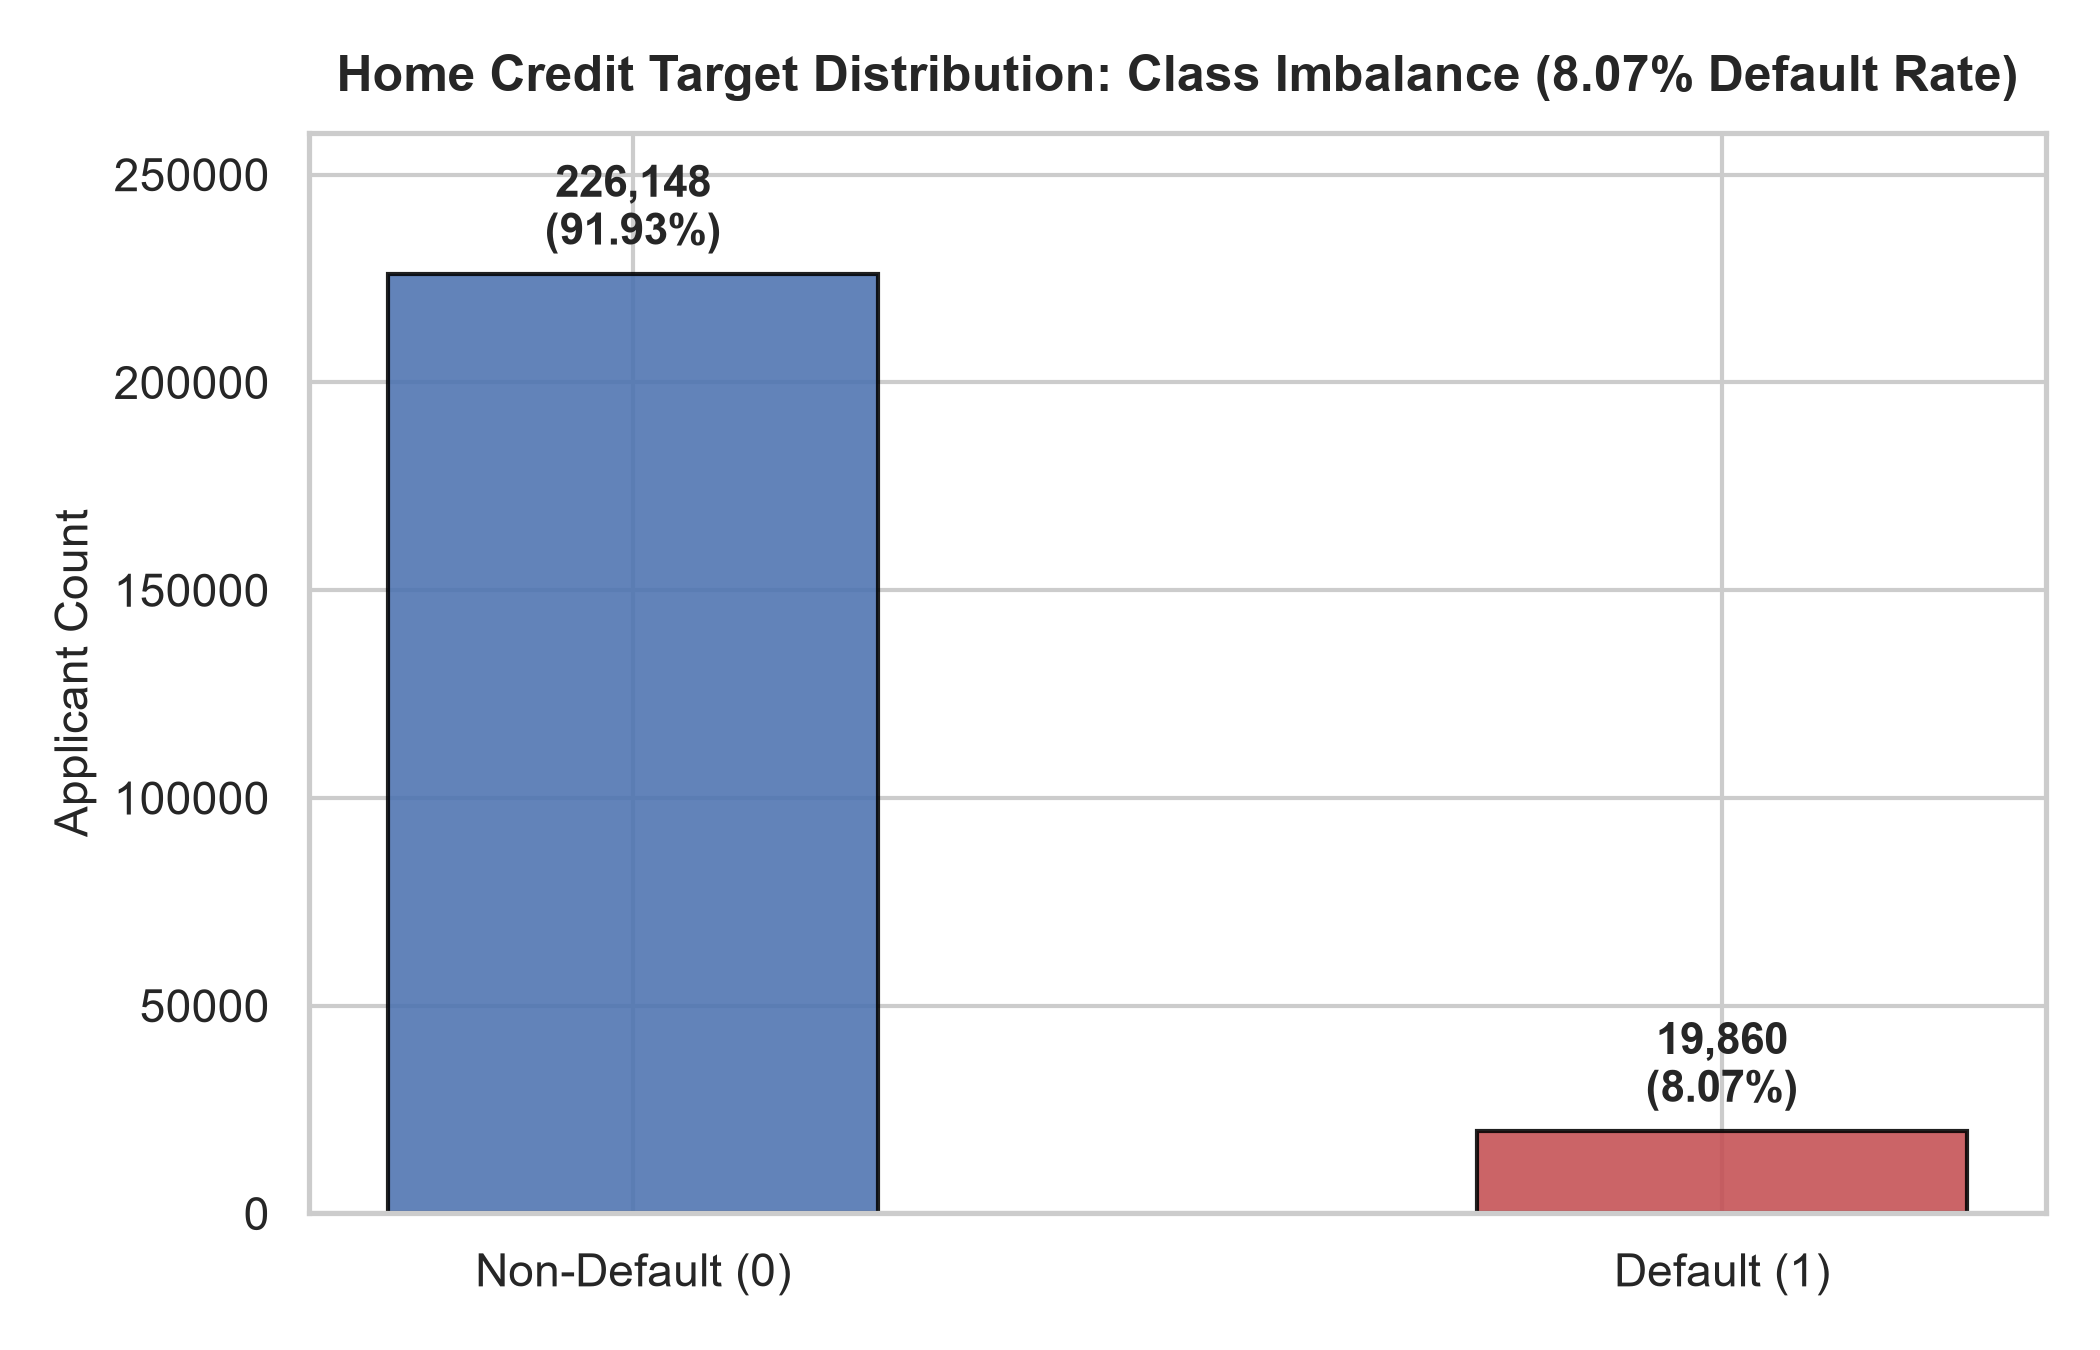
\includegraphics[width=\linewidth,height=1.5in,keepaspectratio]{figures/fig1_target_imbalance.png}
  \vspace{-5pt}
  \caption{\small Target imbalance (8.07\% default) and top missing features.}
\end{minipage}\hfill
\begin{minipage}{0.49\textwidth}
  \centering
  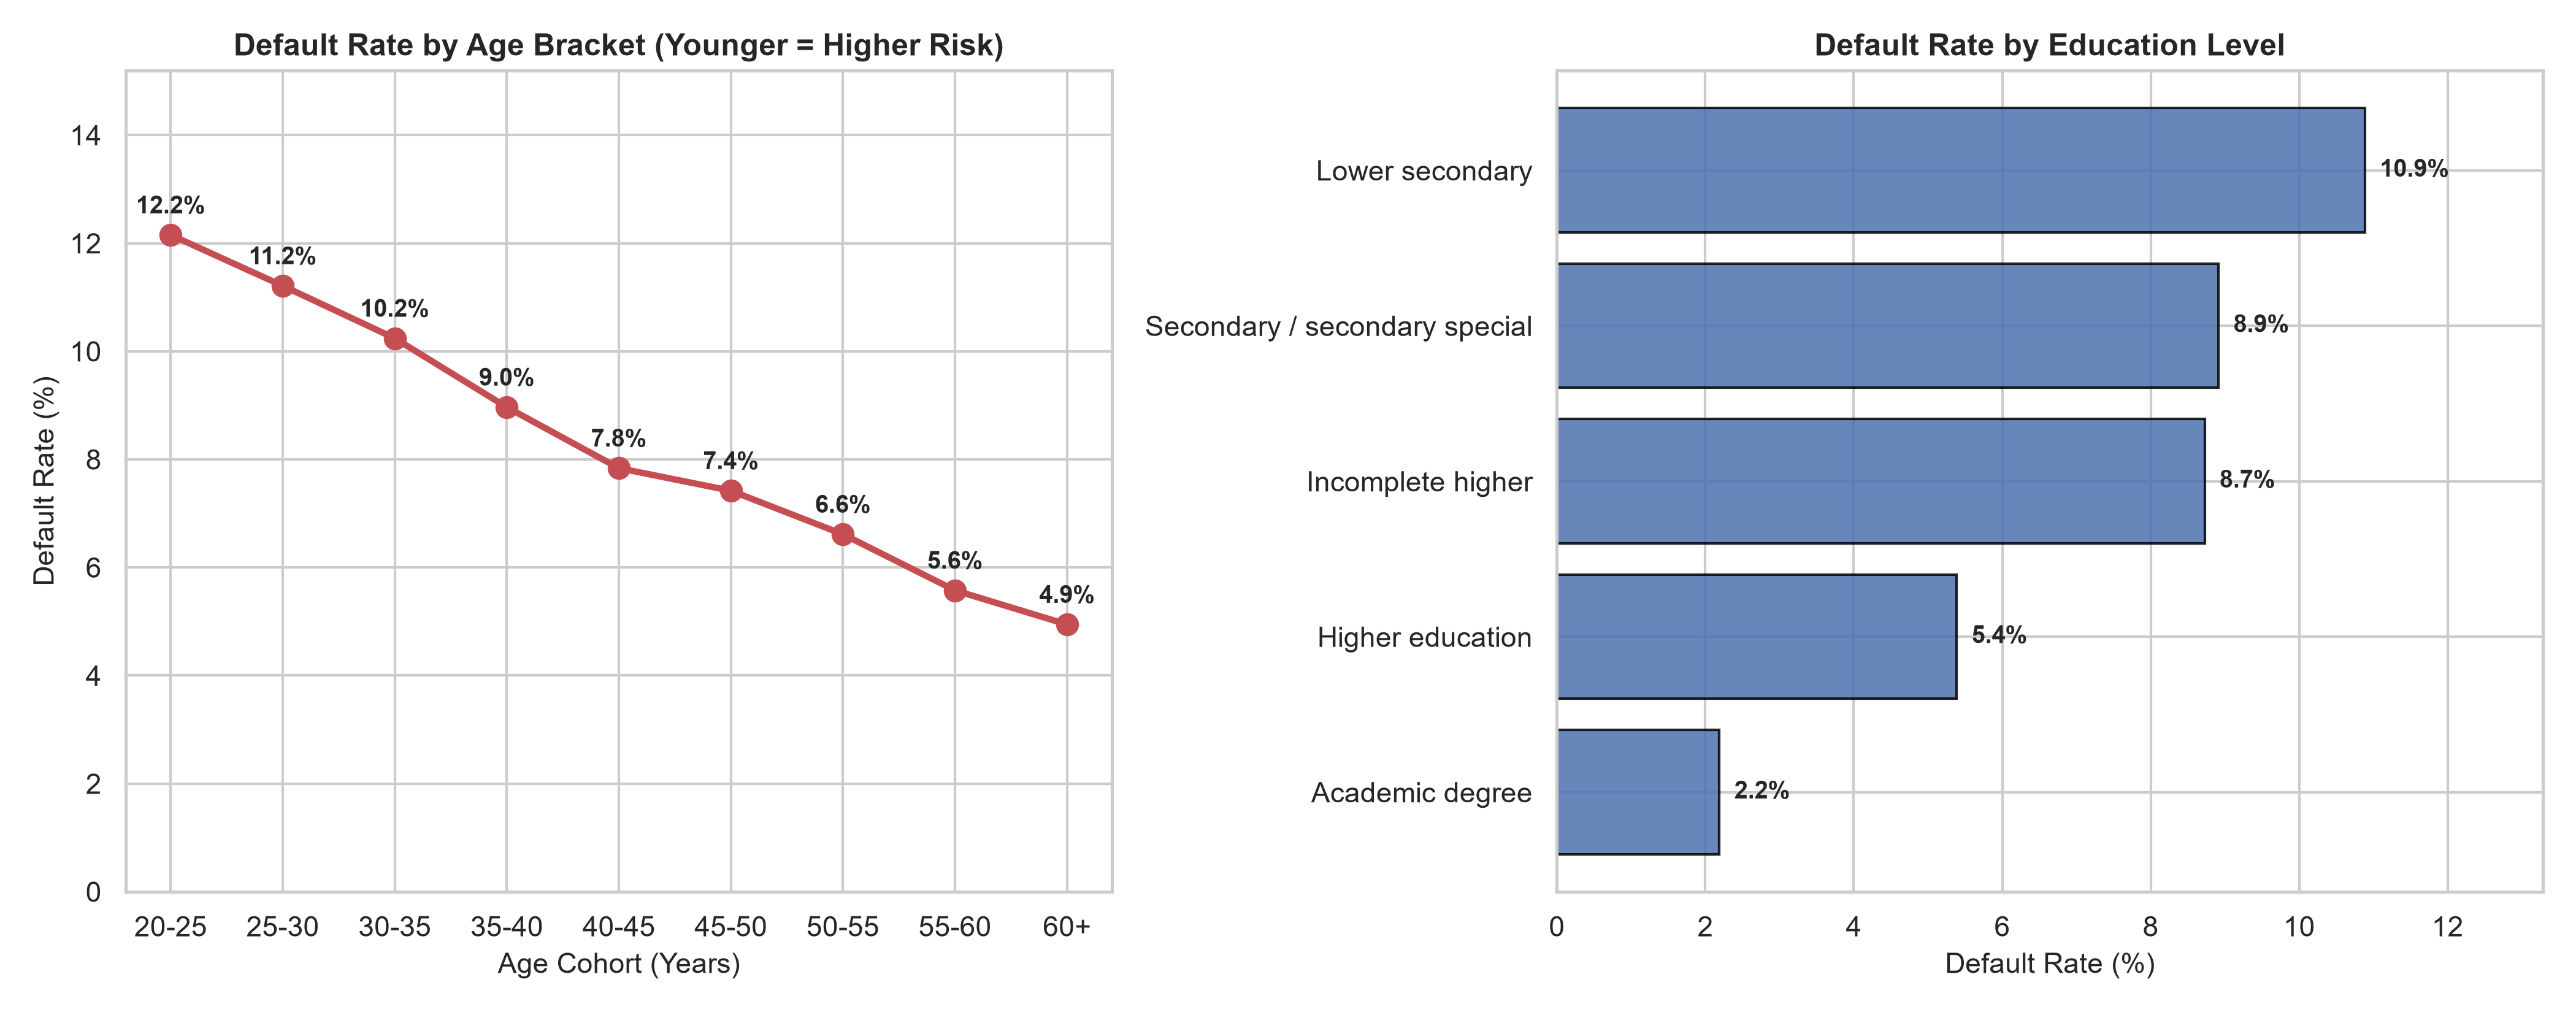
\includegraphics[width=\linewidth,height=1.5in,keepaspectratio]{figures/fig3_demographics_and_age_risk.png}
  \vspace{-5pt}
  \caption{\small Default rate vs. age cohorts: risk drops from 12.3\% to 5.2\%.}
\end{minipage}
\vspace{-6pt}
\end{figure}

\begin{figure}[h!]
\centering
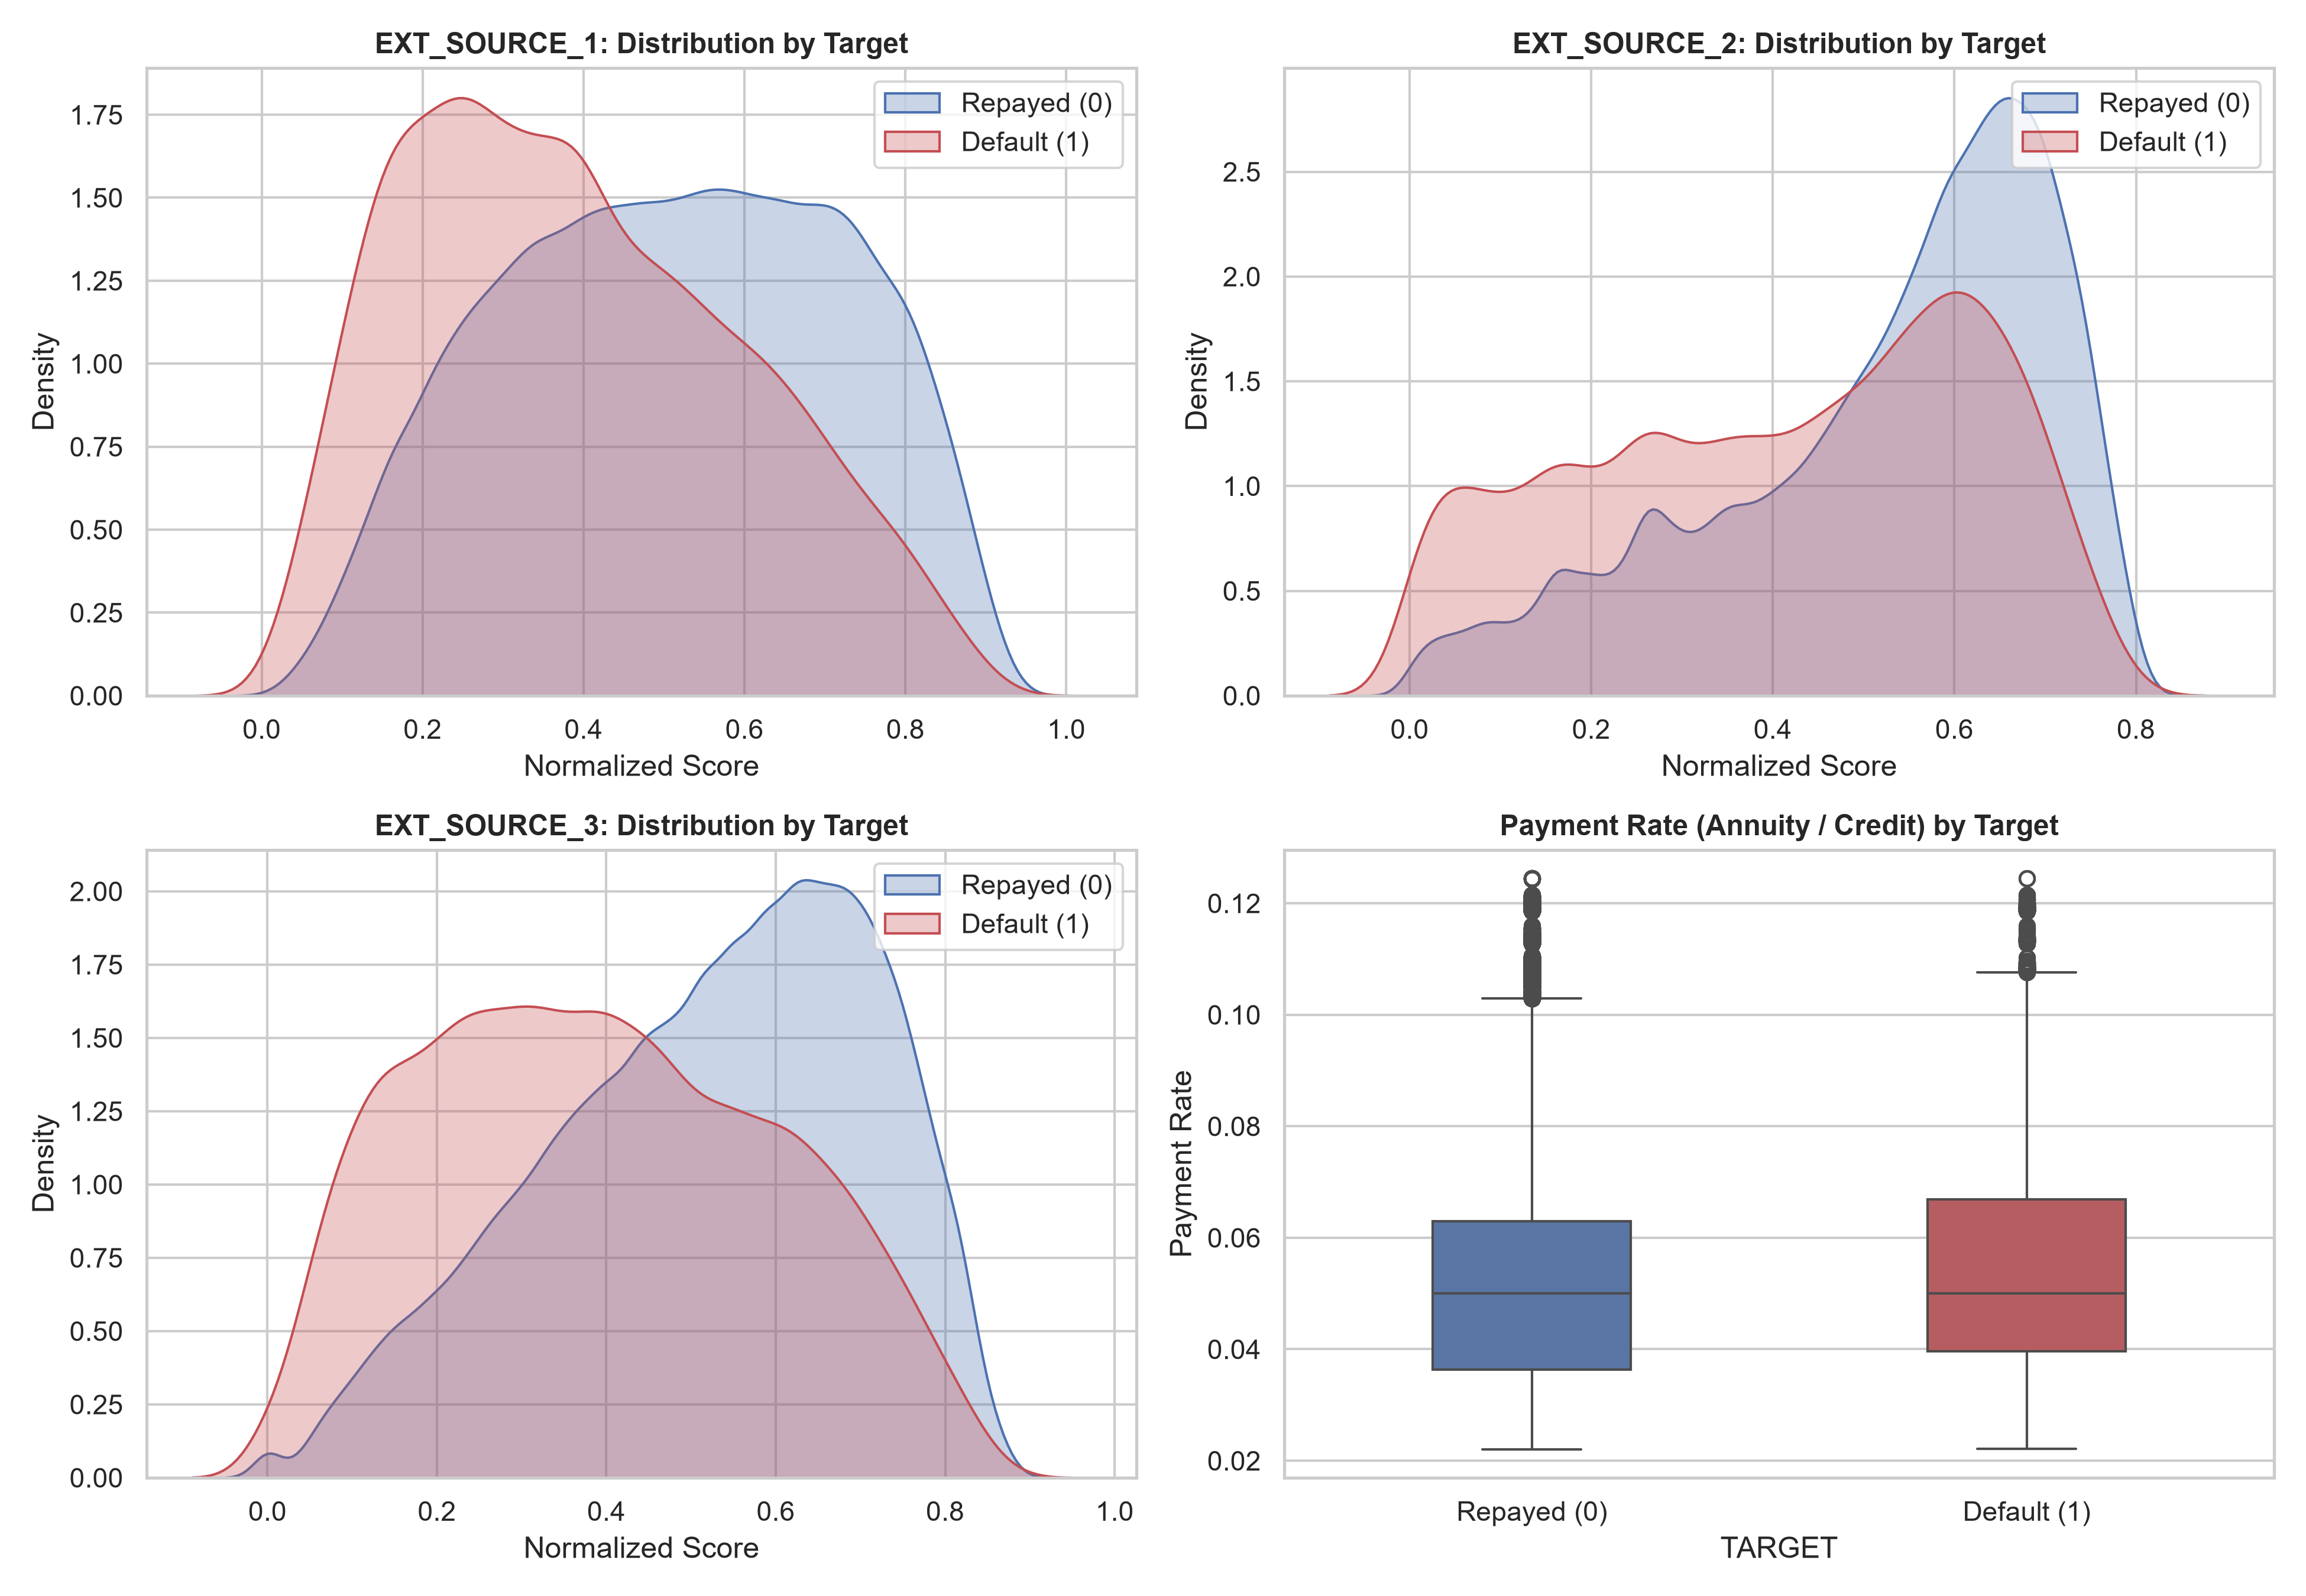
\includegraphics[width=0.76\textwidth,height=1.4in,keepaspectratio]{figures/fig4_financial_ratios_and_ext_kde.png}
\vspace{-5pt}
\caption{\small External bureau score densities (\texttt{EXT\_SOURCE\_1/2/3}) and payment rate distributions across default classes.}
\end{figure}
\vspace{-7pt}

\textbf{Key Analytical Insights:}
\begin{itemize}\setlength{\itemsep}{1pt}\setlength{\parskip}{0pt}
    \item \textbf{External Score Separability}: \texttt{EXT\_SOURCE\_3} ($r = -0.179$), \texttt{EXT\_SOURCE\_2} ($r = -0.161$), and \texttt{EXT\_SOURCE\_1} ($r = -0.155$) exhibit the strongest linear separation with default, confirming bureau scores are informative when available, but leave thin-file applicants unscoreable.
    \item \textbf{Employment Anomaly Divergence}: Applicants with the \texttt{DAYS\_EMPLOYED = 365,243} anomaly exhibit a default rate of only 5.40\% versus 8.66\% for active workers. Explicit flagging prevents models from conflating retired individuals with unstable workers.
    \item \textbf{Age Risk Gradient}: Borrowers aged 20--30 (who predominantly constitute thin-file borrowers) display double the default rate of borrowers aged 60+ (12.3\% vs. 5.2\%), highlighting the critical need for behavioral repayment signals to isolate creditworthy young borrowers.
\end{itemize}

% Section 4
\mysection{4. Data Challenges \& Scaling Solutions}
\begin{itemize}\setlength{\itemsep}{1.5pt}\setlength{\parskip}{0pt}
    \item \textbf{Relational Scale (26.9M Rows) \& Memory Management}: Aggregating four relational tables exceeded standard Colab RAM (12.7 GB). We deployed three mitigations: (1) \textit{Column Pruning}: Loaded raw CSVs using \texttt{usecols} restricted solely to aggregation inputs; (2) \textit{Dtype Downcasting}: Converted \texttt{int64/float64} to smallest safe numeric types (\texttt{int8/16/32}, \texttt{float16/32}) and strings to \texttt{category}, reducing footprints by 30\% to 78.4\% (\texttt{bureau}: 92.7$\rightarrow$42.9 MB [-53.7\%], \texttt{previous\_app}: 66.6$\rightarrow$35.1 MB [-47.7\%], \texttt{POS\_CASH}: 462.4$\rightarrow$100.0 MB [-78.4\%], \texttt{installments}: 544.2$\rightarrow$381.0 MB [-30.0\%]); (3) \textit{Sequential Execution}: Each table was loaded, aggregated, joined, and released via \texttt{del} and \texttt{gc.collect()} before loading the next, staying safely within 12 GB RAM.
    \item \textbf{Temporal Leakage Audit}: Multi-table joins risk lookahead bias. All \texttt{DAYS\_*} and \texttt{MONTHS\_*} fields record negative offsets relative to application date. We asserted and programmatically confirmed non-positive temporal invariants: $\max(\text{DAYS\_CREDIT}) = 0$ (\texttt{bureau}), $\max(\text{DAYS\_INSTALMENT}) = -1$ and $\max(\text{DAYS\_ENTRY\_PAYMENT}) = -1$ (\texttt{installments}), and $\max(\text{MONTHS\_BALANCE}) = -1$ (\texttt{POS\_CASH}). All values $\le 0$, proving zero future leakage. The consolidated matrix was exported to Snappy Parquet (37.3 MB), avoiding repeated joining overhead.
    \item \textbf{Severe Class Imbalance (11.39:1)}: Addressed via cost-sensitive positive class weights (\texttt{scale\_pos\_weight = 11.39}), threshold tuning, and threshold-invariant ranking metrics (ROC-AUC and PR-AUC) rather than deceptive raw accuracy.
\end{itemize}

\newpage
% Section 5
\mysection{5. Methods \& Planned Experiments}

\vspace{1pt}
\noindent\resizebox{\textwidth}{!}{%
\begin{tabular}{@{}llll@{}}
\toprule
\textbf{Model Tier} & \textbf{Model Architecture} & \textbf{Key Hyperparameters \& Tuning Strategy} & \textbf{Role \& Comparison Method} \\
\midrule
\textbf{Baseline} & Regularized Logistic Regression \& & L2 / ElasticNet penalty, standardized inputs, & Establishes linear separability benchmark; \\
 & Shallow Decision Tree & max depth 5, balanced class weights & provides interpretable log-odds baselines. \\
\addlinespace[2pt]
\textbf{Improvement 1} & LightGBM Gradient Boosted & 5-fold Stratified CV; \texttt{scale\_pos\_weight = 11.39}; & Captures high-order non-linear interactions; \\
 & Decision Trees & \texttt{learning\_rate} $\in [0.01, 0.05]$, \texttt{num\_leaves} $\in [31, 63]$ & native missingness routing; SHAP importance. \\
\addlinespace[2pt]
\textbf{Improvement 2} & Deep Tabular Neural Network & Entity Embeddings (categorical) + Dense residual layers; & Learns joint latent representations across \\
 & (TensorFlow / Keras) & Dropout ($p=0.25$), BatchNorm, Adam ($\eta=10^{-3}$), early stop & tabular features; test bed for non-linear embeddings. \\
\bottomrule
\end{tabular}}
\vspace{2pt}

\textbf{Experimental Design \& Validation Framework:}
\begin{itemize}\setlength{\itemsep}{1.5pt}\setlength{\parskip}{0pt}
    \item \textbf{Validation Strategy}: 5-fold Stratified Cross-Validation on the 215,257 training instances; isolated final evaluation on the 61,503 held-out test set.
    \item \textbf{Evaluation Metrics}: Primary discrimination: Area Under the ROC Curve (ROC-AUC); minority detection sensitivity: Area Under the Precision-Recall Curve (PR-AUC); probability calibration: Brier score and expected loss.
    \item \textbf{Subgroup Thin-File Hypothesis Testing}: The test set is partitioned into \textbf{Group A} (traditional applicants with active bureau records, $N \approx 52,000$) and \textbf{Group B} (thin-file applicants lacking bureau history, \texttt{HAS\_BUREAU\_HISTORY = 0}, $N \approx 9,500$). We evaluate models trained on (1) Traditional features, (2) Behavioral alternative features, and (3) Hybrid concatenated features. We test whether the alternative/hybrid lift ($\Delta\text{AUC}$) is statistically significantly larger for Group B using bootstrap confidence intervals ($B = 1,000$).
\end{itemize}

% Section 6
\mysection{6. Team Contributions \& Notebook Ownership Log}
Each team member owns a dedicated notebook with sequentially numbered cells starting at 1, committed to the repository:

\vspace{2pt}
\noindent\resizebox{\textwidth}{!}{%
\begin{tabular}{@{}lllp{6.8in}@{}}
\toprule
\textbf{Team Member} & \textbf{Berkeley Email} & \textbf{Owned Notebook / Track} & \textbf{Specific Milestone Contributions} \\
\midrule
\textbf{Roman Hall} & \texttt{romanhall@berkeley.edu} & \texttt{notebooks/01\_eda\_home\_credit.ipynb} & Static application cleaning, missingness profiling, \texttt{DAYS\_EMPLOYED} anomaly repair, financial burden ratio engineering, generated milestone Figures 1--4, co-authored Sections 1, 2, 3. \\
\addlinespace[2pt]
\textbf{Tung La} & \texttt{tung\_la@berkeley.edu} & \texttt{notebooks/02\_eda\_relational\_tables.ipynb} & Relational aggregation pipeline joining 26.9M rows (\texttt{bureau}, \texttt{previous\_app}, \texttt{POS\_CASH}, \texttt{installments}); memory optimization (\texttt{usecols}, downcasting, sequential GC); Parquet pipeline export; authored Section 4 and co-authored Section 2. \\
\addlinespace[2pt]
\textbf{Faisal Khasawneh} & \texttt{faisal\_k@berkeley.edu} & \texttt{notebooks/03\_alternative\_features.ipynb} & Feature cohort partitioning (Traditional vs. Alternative vs. Hybrid), baseline Logistic Regression scorecard setup, LightGBM tree ensemble tuning harness, co-authored Section 5. \\
\addlinespace[2pt]
\textbf{Advik Goel} & \texttt{advik\_goel@berkeley.edu} & \texttt{notebooks/04\_model\_experiments.ipynb} & TensorFlow deep tabular neural network architecture with entity embeddings, model evaluation pipeline (ROC-AUC, PR-AUC, Brier score), subgroup thin-file evaluation design, co-authored Section 5. \\
\bottomrule
\end{tabular}}

\end{document}
